% Options for packages loaded elsewhere
\PassOptionsToPackage{unicode}{hyperref}
\PassOptionsToPackage{hyphens}{url}
%
\documentclass[
]{article}
\usepackage{amsmath,amssymb}
\usepackage{iftex}
\ifPDFTeX
  \usepackage[T1]{fontenc}
  \usepackage[utf8]{inputenc}
  \usepackage{textcomp} % provide euro and other symbols
\else % if luatex or xetex
  \usepackage{unicode-math} % this also loads fontspec
  \defaultfontfeatures{Scale=MatchLowercase}
  \defaultfontfeatures[\rmfamily]{Ligatures=TeX,Scale=1}
\fi
\usepackage{lmodern}
\ifPDFTeX\else
  % xetex/luatex font selection
\fi
% Use upquote if available, for straight quotes in verbatim environments
\IfFileExists{upquote.sty}{\usepackage{upquote}}{}
\IfFileExists{microtype.sty}{% use microtype if available
  \usepackage[]{microtype}
  \UseMicrotypeSet[protrusion]{basicmath} % disable protrusion for tt fonts
}{}
\makeatletter
\@ifundefined{KOMAClassName}{% if non-KOMA class
  \IfFileExists{parskip.sty}{%
    \usepackage{parskip}
  }{% else
    \setlength{\parindent}{0pt}
    \setlength{\parskip}{6pt plus 2pt minus 1pt}}
}{% if KOMA class
  \KOMAoptions{parskip=half}}
\makeatother
\usepackage{xcolor}
\usepackage[margin=1in]{geometry}
\usepackage{graphicx}
\makeatletter
\def\maxwidth{\ifdim\Gin@nat@width>\linewidth\linewidth\else\Gin@nat@width\fi}
\def\maxheight{\ifdim\Gin@nat@height>\textheight\textheight\else\Gin@nat@height\fi}
\makeatother
% Scale images if necessary, so that they will not overflow the page
% margins by default, and it is still possible to overwrite the defaults
% using explicit options in \includegraphics[width, height, ...]{}
\setkeys{Gin}{width=\maxwidth,height=\maxheight,keepaspectratio}
% Set default figure placement to htbp
\makeatletter
\def\fps@figure{htbp}
\makeatother
\setlength{\emergencystretch}{3em} % prevent overfull lines
\providecommand{\tightlist}{%
  \setlength{\itemsep}{0pt}\setlength{\parskip}{0pt}}
\setcounter{secnumdepth}{-\maxdimen} % remove section numbering
\usepackage{multicol}
\usepackage{longtable}
\setlength{\columnsep}{1cm}
\usepackage{booktabs}
\usepackage{array}
\usepackage{float}
\usepackage{longtable}
\usepackage{multirow}
\usepackage{wrapfig}
\usepackage{colortbl}
\usepackage{pdflscape}
\usepackage{tabu}
\usepackage{threeparttable}
\usepackage{threeparttablex}
\usepackage[normalem]{ulem}
\usepackage{makecell}
\usepackage{xcolor}
\ifLuaTeX
  \usepackage{selnolig}  % disable illegal ligatures
\fi
\usepackage{bookmark}
\IfFileExists{xurl.sty}{\usepackage{xurl}}{} % add URL line breaks if available
\urlstyle{same}
\hypersetup{
  pdftitle={Análisis de Variables que Influyen en la Inversión, Innovación e Implementación de la Inteligencia Artificial},
  hidelinks,
  pdfcreator={LaTeX via pandoc}}

\title{Análisis de Variables que Influyen en la Inversión, Innovación e
Implementación de la Inteligencia Artificial}
\author{Adrada Isabel, De la Peña Juan, Terán Federico, Troncoso
Samuel\\
Pontificia Universidad Javeriana Cali}
\date{}

\begin{document}
\maketitle

\begin{multicols}{2}

\section{Resumen}
...
...

\section{Key words}
...
...

\section{Introducción}
Las compañıas involucradas en el desarrollo tecnológico con inteligencia artificial (IA) necesitan identificar las regiones con mayor potencial de adopción e implementación de estas herramientas. Este análisis es crucial para la toma de decisiones estratégicas, la definición de mercados objetivo y la planificación de estrategias de expansión geográfica, razón por lo cuál, debido a la incertidumbre respecto a los factores con mayor impacto en el potencial éxito de los planes de expansión operativa en diferentes partes del mundo, se plantea el interrogante ¿Qué variables tienen mayor influencia en los niveles de inversión, innovación e implementación de la inteligencia artificial según lo reflejado en el AI Global Index [1] (índice que compara diferentes países en estos niveles), y cómo varía esta influencia según la región geográfica?.

El objetivo general de este estudio radica en identificar las variables con un mayor grado de influencia en el nivel de inversión, innovación e implementación de la inteligencia artificial, reflejado en el AI global index de diferentes regiones del mundo, por lo cuál, en primera instancia se identificaron los índices para cada factor mencionado con un mayor coeficiente de correlación lineal de Pearson de acuerdo a la metodología e interpretación plaenteada por Navidi [2], permitiendo el plateamiento de los objetivos específicos con el fin de determinar la influencia de los factores relacionados con la inversión mediante el índice Commerce, la innovación mediante el índice Research, la implementación mediante el índice Talent y la ubicación geográfica del país mediante la categorización por Región.

A partir de los anteriores planteamientos se formula como hipótesis: la influencia del nivel de inversión (índice Commerce), innovación (índice Research) e implementación (índice Talent) de inteligencia artificial en el desempeño de los países según el AI Global Index (Total Score) presenta diferencias altamente significativas según la región geográfica.




\section{Métodos}
Para la definición de las variables a estudiar a partir de la base de datos AI Global Index trabajada en el presente estudio, se relalizó una exploración preliminar de los datos en la Tabla 1, donde se nombran las variables, se clasifican como cualitativas o cuantitativas, se categorizan como continuas o discretas, o nominal u ordinal según el caso y se realiza una descripción de las mismas.

\end{multicols}

\renewcommand{\arraystretch}{1.5}
\begin{footnotesize}
\begin{longtable}[t]{lllp{8cm}}
\caption{\label{tab:tabla1}Variables y su clasificación}\\
\toprule
Variable & Clasificación & Categorización & Descripción\\
\midrule
Country & Cualitativa & Nominal & Nombre del país donde se evalúa el AI Global Index.\\
Talent & Cuantitativa & Continua & Indicador de disponibilidad de profesionales calificados para la provisión de soluciones de inteligencia artificial.\\
Infraestructure & Cuantitativa & Continua & Indicador de fiabilidad y la escala de la infraestructura de acceso, desde la electricidad e Internet, hasta las capacidades de superintarmética.\\
Operating Enviroment & Cuantitativa & Continua & Indicador del contexto regulatorio y la opinión pública en torno a la inteligencia artificial.\\
Research & Cuantitativa & Continua & Indicador del alcance de la investigación especializada y los investigadores; investigando la cantidad de publicaciones y citas en revistas académicas creíbles.\\
\addlinespace
Development & Cuantitativa & Continua & Indicador de desarrollo de plataformas y algoritmos fundamentales en los que se basan los proyectos innovadores de inteligencia artificial.\\
Government Strategy & Cuantitativa & Continua & Indicador de la profundidad del compromiso del gobierno nacional con la inteligencia artificial; investigando los compromisos de gasto y las estrategias nacionales.\\
Commercial & Cuantitativa & Continua & Indicador del nivel de actividad de puesta en marcha, inversión e iniciativas comerciales basadas en la inteligencia artificial.\\
Total Score & Cuantitativa & Continua & Indicador AI Global Index que compara a las naciones en su nivel de inversión, innovación e implementación de la inteligencia artificial.\\
Region & Cualitativa & Nominal & Agrupacion de países según su localización geográfica en regiones.\\
\addlinespace
Cluster & Cualitativa & Nominal & Agrupación de países según su historia de incursión en el desarrollo de tecnología relacionada con la Inteligencia Artificial.\\
Income Group & Cualitativa & Ordinal & Nivel de ingresos presentado en el país.\\
Political Regime & Cualitativa & Nominal & Tipo de régimen político presentado en el país.\\
\bottomrule
\end{longtable}

\end{footnotesize}\renewcommand{\arraystretch}{1}

\begin{multicols}{2}


Posteriormente, con el propósito de indentificar las posibles variables con un mayor grado de influencia en el nivel de inversión, innovación e implementación de la inteligencia artificial, se elaboró la figura 1, la cuál presenta una comparación de las distribuciones de las variables y sus respectivos coeficientes de correlación lineal de Pearson con el fin de reconocer los índices que presentan un mayor valor respecto al AI Global Index (Total Score), los cuáles fueron Commerce para el nivel de inversión, Research para la innovación y Talent para la implemetación. 




\begin{center}
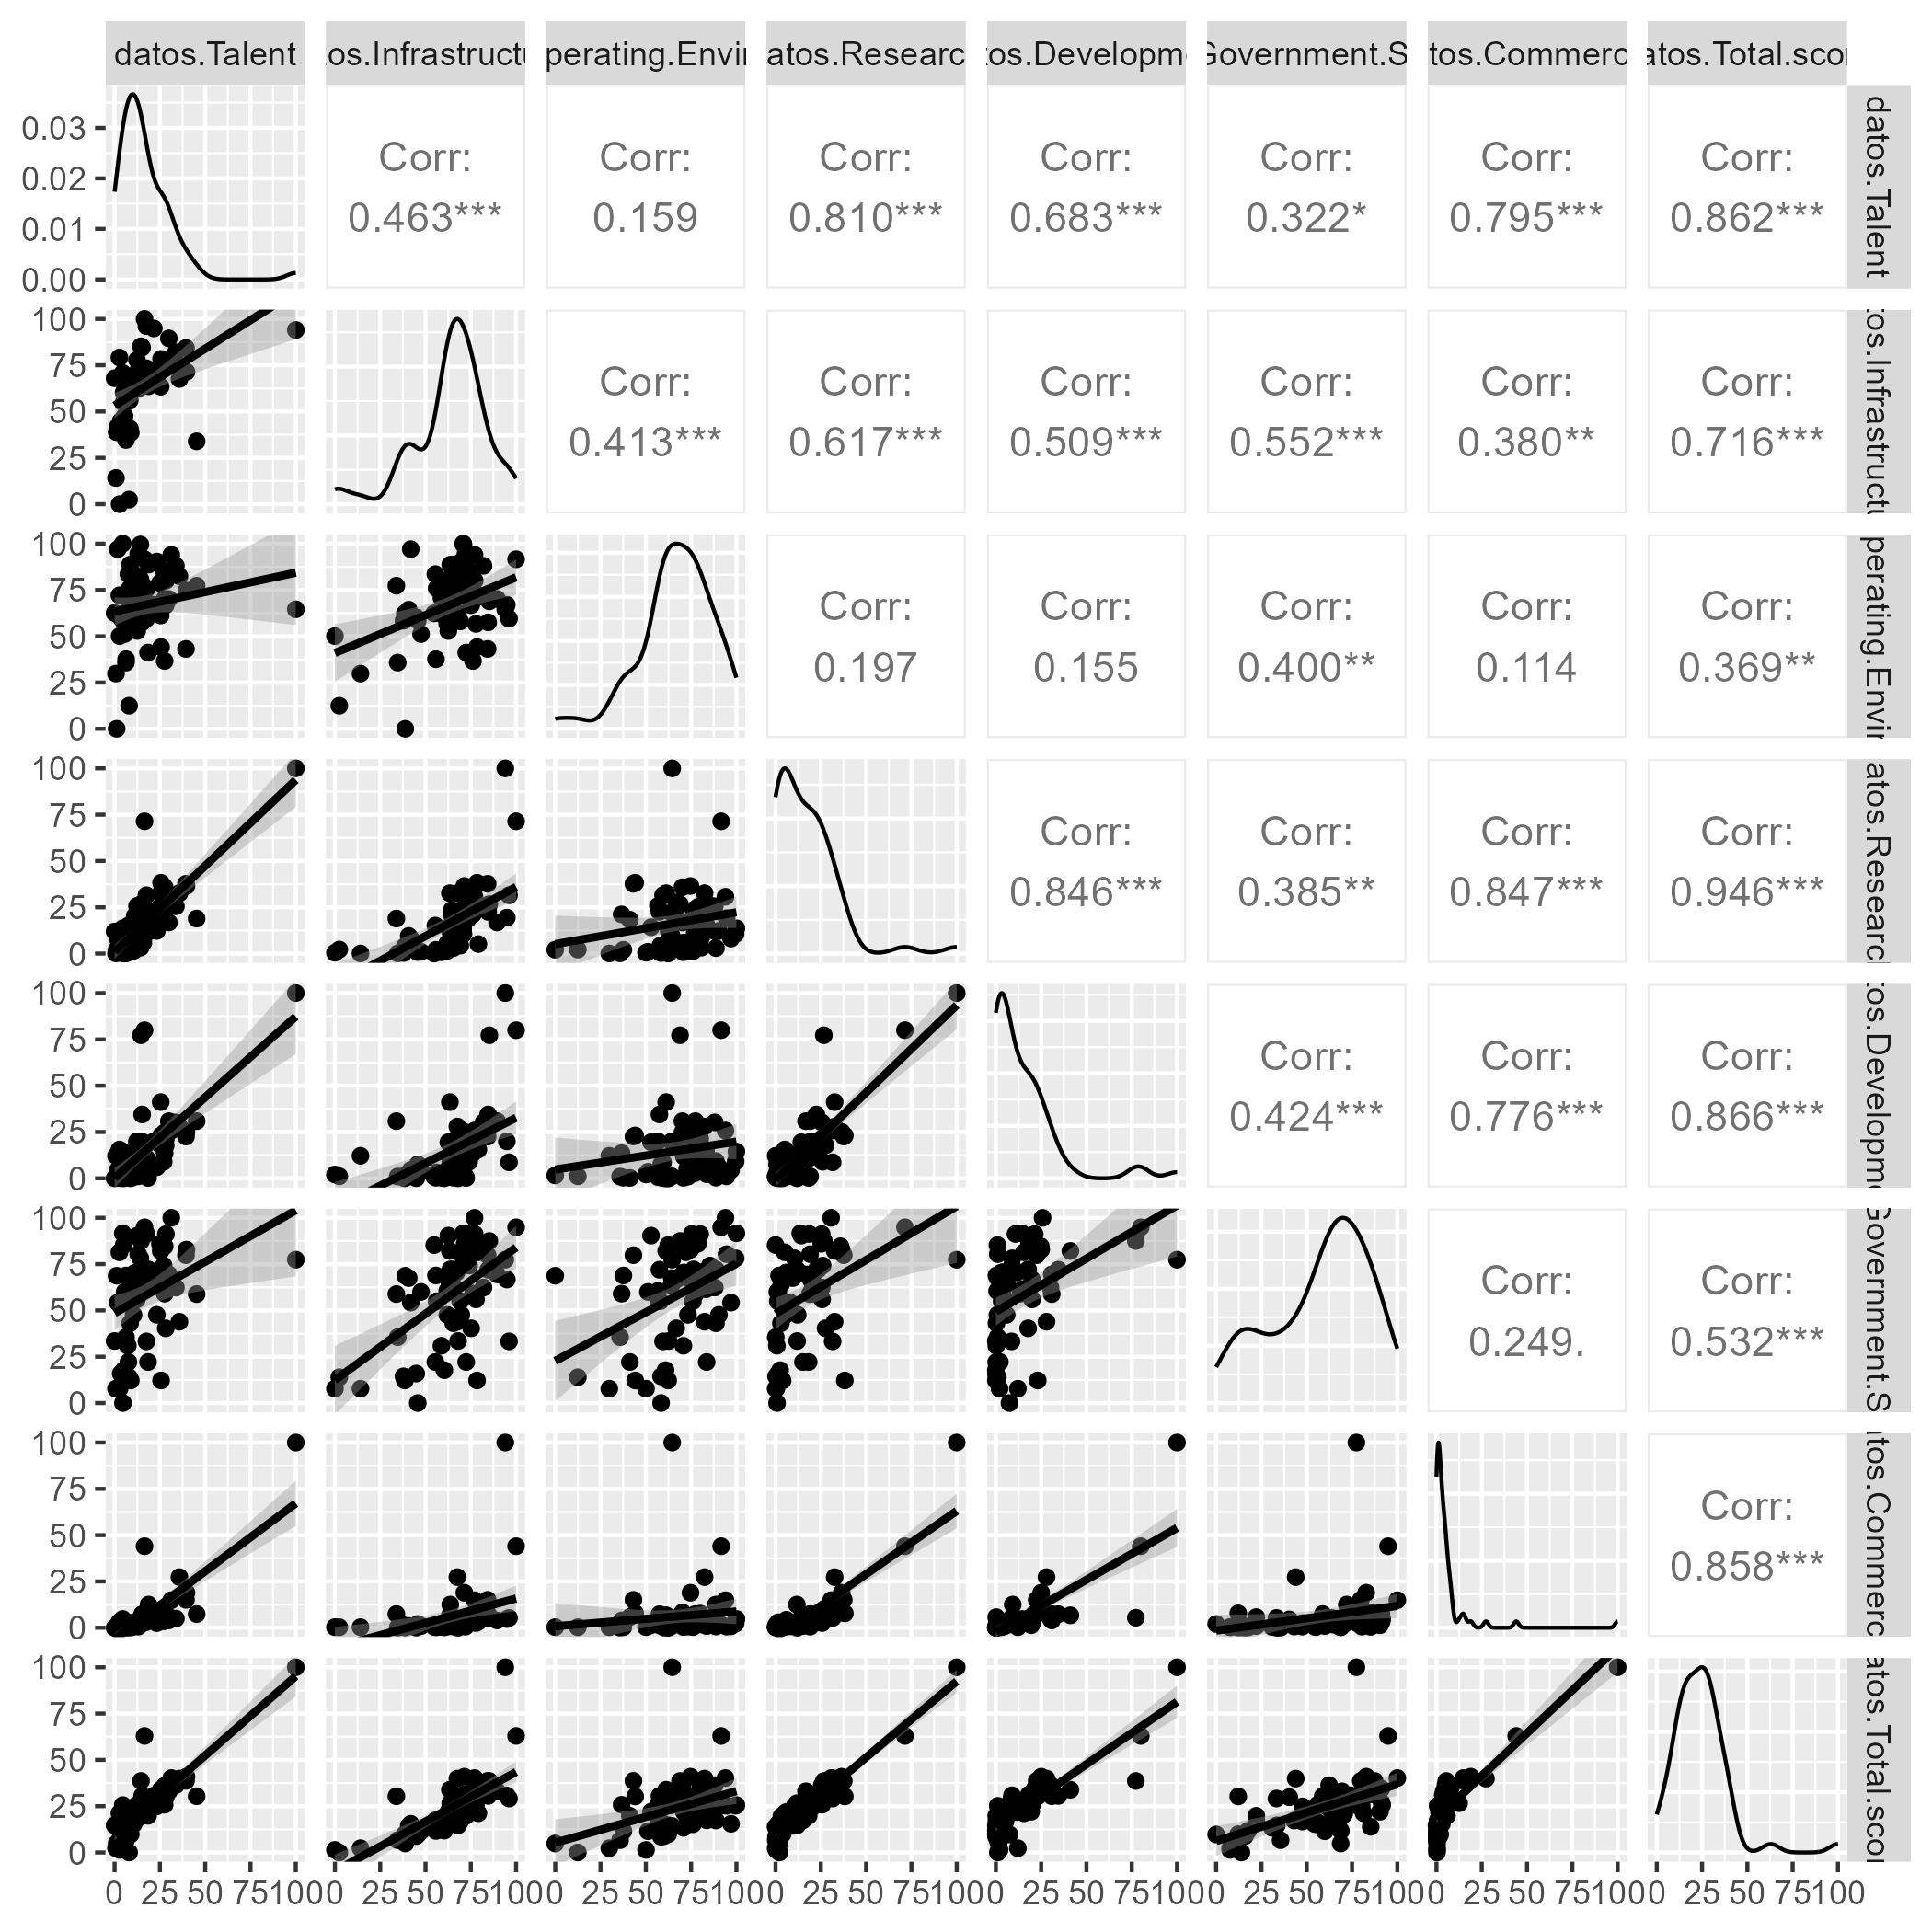
\includegraphics[width=\linewidth]{figura1.png}
\end{center}
Figura 1. Correlación lineal de Pearson índices.

Posteriormente, se realizó ... 
... para cada uno de los índices con el fin de ...

\section{Resultados}
En la Tabla 2 se presentan las medidas de tendencia central y posición de las variables cuantitativas Índice Commerce, Research y Talent discriminadas de forma regional. 

Para casi todos los casos, la medida de tendencia central moda presentó más de tres valores, lo cuál no brinda mucha información acerca de los datos. En el caso de la media y mediana en Americas y Middle East, todos los índices difieren drásticamente, lo cuál indica que la distribución de los datos no es normal. En el caso Asia-Pacific, para el indicador Research y Total Score hay una alta cercanía entre estos indicadores, planteando la posibilidad de una distribución de campana. Esto mismo ocurre para Europe con todos los indicadores, y en el caso del indicador Commerce hay una moda única que también es significativamente cercana a la media y mediana. Finalmente para Africa se presenta una alta cercanía de la mediana y la media en los índices Commerce, Talent y Research.

El mínimo en todas las regiones para todos los ídices es menor a 10, excepto Total Score de Americas con un 13.27, por otro lado, el máximo entre regiones presenta discrepancias más significativas, donde el el caso de Americas el máximo es 100 para todos los índices, en Asia-Pacific todos los máximos se encuentran por encima de 40, mientras en Europe los máximos de todos los índices se ubican en 40.93 o menos, al igual que Middle East. En el caso de Africa, toos los máximos de los indicadores se encuentran por debajo de 10.

\end{multicols}

\renewcommand{\arraystretch}{1.3}
\begin{scriptsize}
\begin{longtable}[t]{llrrrrrrr}
\caption{\label{tab:tabla2}Medidas de tendencia central y posición}\\
\toprule
Región & Índice & Media & Moda & Mínimo & Q1 & Mediana & Q3 & Máximo\\
\midrule
Americas & Commerce & 15.15 & > 3 modas & 0.34 & 0.48 & 1.07 & 5.93 & 100.00\\
Americas & Talent & 22.21 & > 3 modas & 1.72 & 6.70 & 9.48 & 17.91 & 100.00\\
Americas & Research & 18.39 & > 3 modas & 0.00 & 1.12 & 3.16 & 13.75 & 100.00\\
Americas & Total Score & 29.03 & > 3 modas & 13.27 & 14.89 & 15.41 & 24.22 & 100.00\\
Asia-Pacific & Commerce & 7.03 & > 3 modas & 0.09 & 0.70 & 3.92 & 7.16 & 44.02\\
\addlinespace
Asia-Pacific & Talent & 17.58 & > 3 modas & 5.51 & 8.61 & 14.86 & 21.87 & 45.27\\
Asia-Pacific & Research & 20.72 & > 3 modas & 0.12 & 3.02 & 20.72 & 30.30 & 71.42\\
Asia-Pacific & Total Score & 25.79 & > 3 modas & 0.00 & 12.88 & 27.45 & 33.03 & 62.92\\
Europe & Commerce & 4.28 & 3.08 & 0.61 & 1.75 & 3.46 & 4.97 & 18.91\\
Europe & Talent & 18.92 & > 3 modas & 6.69 & 12.46 & 16.97 & 27.07 & 39.65\\
\addlinespace
Europe & Research & 17.86 & > 3 modas & 0.28 & 10.60 & 18.60 & 25.21 & 38.24\\
Europe & Total Score & 25.49 & > 3 modas & 8.49 & 20.31 & 25.52 & 30.73 & 40.93\\
Middle East & Commerce & 5.97 & > 3 modas & 0.00 & 0.26 & 1.77 & 4.35 & 27.33\\
Middle East & Talent & 8.17 & > 3 modas & 0.00 & 1.50 & 3.57 & 4.86 & 35.76\\
Middle East & Research & 11.32 & > 3 modas & 2.08 & 3.18 & 8.54 & 13.21 & 32.63\\
\addlinespace
Middle East & Total Score & 19.66 & > 3 modas & 4.83 & 12.51 & 17.91 & 24.49 & 39.89\\
Africa & Commerce & 0.58 & > 3 modas & 0.10 & 0.15 & 0.31 & 0.33 & 2.03\\
Africa & Talent & 4.08 & > 3 modas & 0.75 & 2.74 & 3.36 & 4.61 & 8.94\\
Africa & Research & 1.34 & > 3 modas & 0.07 & 0.45 & 0.83 & 1.46 & 3.90\\
Africa & Total Score & 6.43 & > 3 modas & 1.38 & 2.30 & 8.87 & 9.71 & 9.87\\
\bottomrule
\end{longtable}

\end{scriptsize}\renewcommand{\arraystretch}{1}

\begin{multicols}{2}

En la Tabla 3 se presentan las medidas de disperción, covarianza y correlación lineal de Pearson con respecto al Total Score (AI Global Index) de las variables cuantitativas Índice Commerce, Research y Talent discriminadas de forma regional. 

Americas presentan los rangos más amplios de todas las regiones que van desde 86.73 en Total Score hasta 100 en Research, para la maroría los demás casos de las regiones Asia-Pacific, Europe y Middle East, los rangos de los diferentes índices varían alrededor de 20 y 40 indicando menor variablidad de los datos con excepciones de los índices Research y Total Score de Asia-Pacific con 71.30 y  62.92 respectivamente. En el caso de Africa se presentan los rangos más bajos donde todos estàn por debajo de 10, lo cuál sugiere que los datos en la región se distribuyen de manera altamente compacta.

Con respecto al coeeficiente de variación se puede afirmar que para la mayoría de los casos los datos son heterogéneos al presentar un coeficiente de variación mayor a 50, sin embargo, el índice Talent y Total Score en Europe presentan variación significativa ya que el coeficiente de variación se encuentra en el rango de 10 a 50.

En el caso de la covarianza, esta es positiva para todas las variables, lo cuál plantea la posibilidad de que estas tengan una relación lineal directa con el índice Total Score. Esto es confirmado con el coeficiente de correlación de Pearson, donde un valor superior a 0.8 indica hay una relación muy significativa, lo cuál es cierto para todos los indicadores en Americas y Middle East, Research en Asia-Pacific y Talent y Research en Europe. Por otro lado, una coeficiente entre 0.6 y 0.78 indica una relación significativa, la cuál está presente en Europe para el indicador Commerce y en Africa para Talent y Research.


\end{multicols}

\renewcommand{\arraystretch}{1.3}
\begin{scriptsize}
\begin{longtable}[t]{llrrrrrl}
\caption{\label{tab:tabla3}Medidas de dispersión e indicadores por región e índice}\\
\toprule
Región & Índice & Rango & RIQ & Desv.est & CV & Cov Total Score & Corr Total Score\\
\midrule
Americas & Commerce & 99.66 & 5.45 & 34.63 & 228.58 & 1025.58 & 0.99\\
Americas & Talent & 98.28 & 11.21 & 32.68 & 147.14 & 976.48 & 1.00\\
Americas & Research & 100.00 & 12.63 & 34.50 & 187.60 & 1033.01 & 1.00\\
Americas & Total Score & 86.73 & 9.33 & 30.01 & 103.38 & 900.62 & 1.00\\
Asia-Pacific & Commerce & 43.93 & 6.46 & 11.43 & 162.59 & 154.14 & 0.84\\
\addlinespace
Asia-Pacific & Talent & 39.76 & 13.26 & 12.16 & 69.17 & 95.12 & 0.49\\
Asia-Pacific & Research & 71.30 & 27.28 & 19.60 & 94.59 & 298.15 & 0.95\\
Asia-Pacific & Total Score & 62.92 & 20.15 & 16.05 & 62.23 & 257.75 & 1.00\\
Europe & Commerce & 18.30 & 3.22 & 3.92 & 91.59 & 19.30 & 0.67\\
Europe & Talent & 32.96 & 14.61 & 8.71 & 46.04 & 57.84 & 0.91\\
\addlinespace
Europe & Research & 37.96 & 14.61 & 10.12 & 56.66 & 61.59 & 0.83\\
Europe & Total Score & 32.44 & 10.42 & 7.33 & 28.76 & 53.68 & 1.00\\
Middle East & Commerce & 27.33 & 4.09 & 10.64 & 178.22 & 115.90 & 0.89\\
Middle East & Talent & 35.76 & 3.37 & 13.65 & 167.07 & 139.71 & 0.83\\
Middle East & Research & 30.55 & 10.03 & 11.50 & 101.59 & 127.72 & 0.90\\
\addlinespace
Middle East & Total Score & 35.06 & 11.98 & 12.28 & 62.46 & 150.74 & 1.00\\
Africa & Commerce & 1.93 & 0.18 & 0.81 & 139.66 & 1.12 & 0.33\\
Africa & Talent & 8.19 & 1.87 & 3.05 & 74.75 & 9.30 & 0.72\\
Africa & Research & 3.83 & 1.01 & 1.52 & 113.43 & 4.29 & 0.67\\
Africa & Total Score & 8.49 & 7.41 & 4.22 & 65.63 & 17.78 & 1.00\\
\bottomrule
\end{longtable}

\end{scriptsize}\renewcommand{\arraystretch}{1}

\begin{multicols}{2}

...

\subsection{Índice Commerce}

En la Tabla 4 se presentan las frecuencias bivariadas del indice Commerce y el índice Total Score, 

\end{multicols}

\renewcommand{\arraystretch}{1.3}
\begin{footnotesize}\begin{table}[!h]
\centering
\caption{\label{tab:tabla4}Tabla de Frecuencia Bivariada Índice Commerce (A) vs Total Score (B)}
\centering
\resizebox{\ifdim\width>\linewidth\linewidth\else\width\fi}{!}{
\begin{tabular}[t]{lrrrrrrrrrrr}
\toprule
A   \textbackslash{}   B & (0, 10] & (10, 20] & (20, 30] & (30, 40] & (40, 50] & (50, 60] & (60, 70] & (70, 80] & (80, 90] & (90, 100] & Total\\
\midrule
(0, 10] & 9 & 17 & 17 & 12 & 0 & 0 & 0 & 0 & 0 & 0 & 55\\
(10, 20] & 0 & 0 & 1 & 1 & 2 & 0 & 0 & 0 & 0 & 0 & 4\\
(20, 30] & 0 & 0 & 0 & 1 & 0 & 0 & 0 & 0 & 0 & 0 & 1\\
(30, 40] & 0 & 0 & 0 & 0 & 0 & 0 & 0 & 0 & 0 & 0 & 0\\
(40, 50] & 0 & 0 & 0 & 0 & 0 & 0 & 1 & 0 & 0 & 0 & 1\\
\addlinespace
(50, 60] & 0 & 0 & 0 & 0 & 0 & 0 & 0 & 0 & 0 & 0 & 0\\
(60, 70] & 0 & 0 & 0 & 0 & 0 & 0 & 0 & 0 & 0 & 0 & 0\\
(70, 80] & 0 & 0 & 0 & 0 & 0 & 0 & 0 & 0 & 0 & 0 & 0\\
(80, 90] & 0 & 0 & 0 & 0 & 0 & 0 & 0 & 0 & 0 & 0 & 0\\
(90, 100] & 0 & 0 & 0 & 0 & 0 & 0 & 0 & 0 & 0 & 1 & 1\\
\addlinespace
Total & 9 & 17 & 18 & 14 & 2 & 0 & 1 & 0 & 0 & 1 & 62\\
\bottomrule
\end{tabular}}
\end{table}
\end{footnotesize}\renewcommand{\arraystretch}{1}

\begin{multicols}{2}

El histograma presentado en la Figura 2 permite plasmar gráficamente la distribución de los datos de la variable índince Commerce. Su puede observar como en los casos de Americas, Asia-Pacific y Middle East los datos se encuentran concentrados hacia la izquierda del eje x, sin embargo presentan una asimetría positiva o sesgo a la derecha, donde la media es mayor a la mediana, indicando que posiblemente se presenten puntos atípicos hacia la derecha del eje x.

En el caso de Europe, se observa que los datos se agrupan hacia la izquierda del eje x, sin embarrgo, aunque en el análisis de la Tabla 2 se teorizaba una posible distribución normal debido a la cercanía de la media, mediana y moda, no se muestra simetría en la gráfica,ya que esta muestra una distribución con mayor similitud a una exponencial.

En el caso de Africa, los datos se encuentran concentrados alrededor del 0




\begin{center}
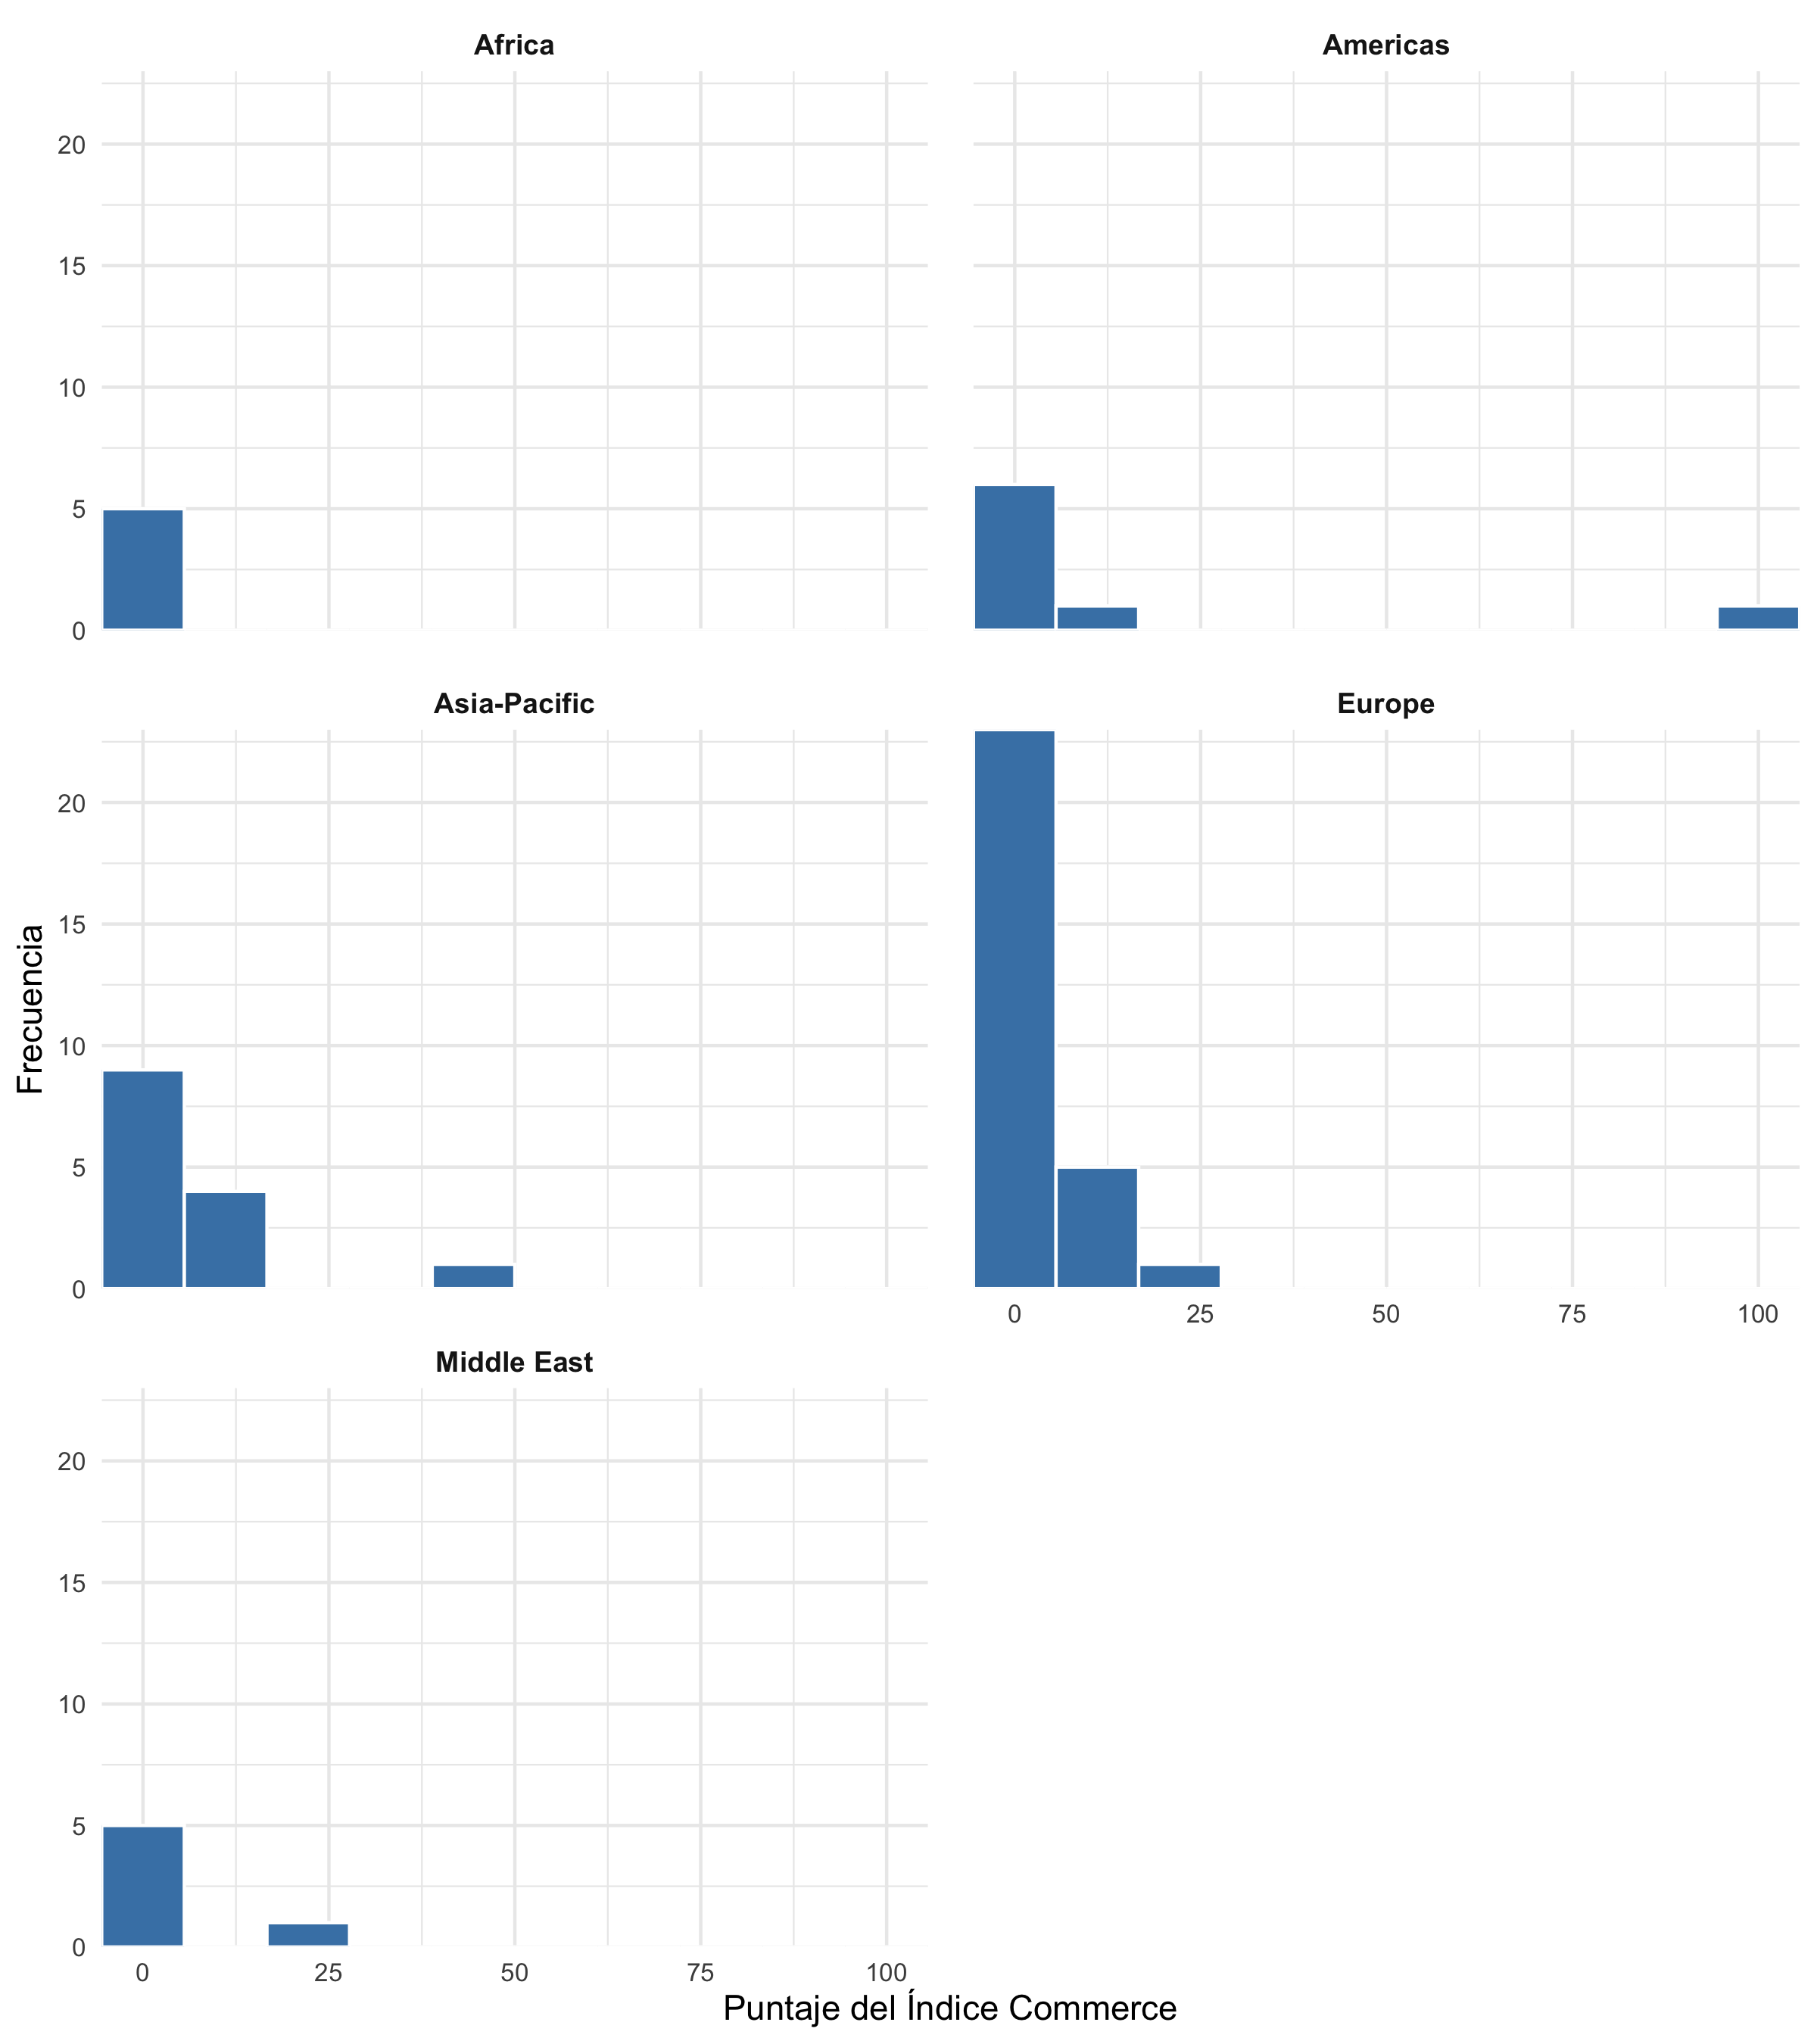
\includegraphics[width=\linewidth]{figura2.png}
\end{center}
Figura 2. Distribución del Índice Commerce agrupado por Región.


La Ojiva en la Figura 3 presenta la distriución acumulada de los datos de manera porcental, lo cuál permite estimar los percentiles correspondientes a los diferentes puntajes del índice Commerce



\begin{center}
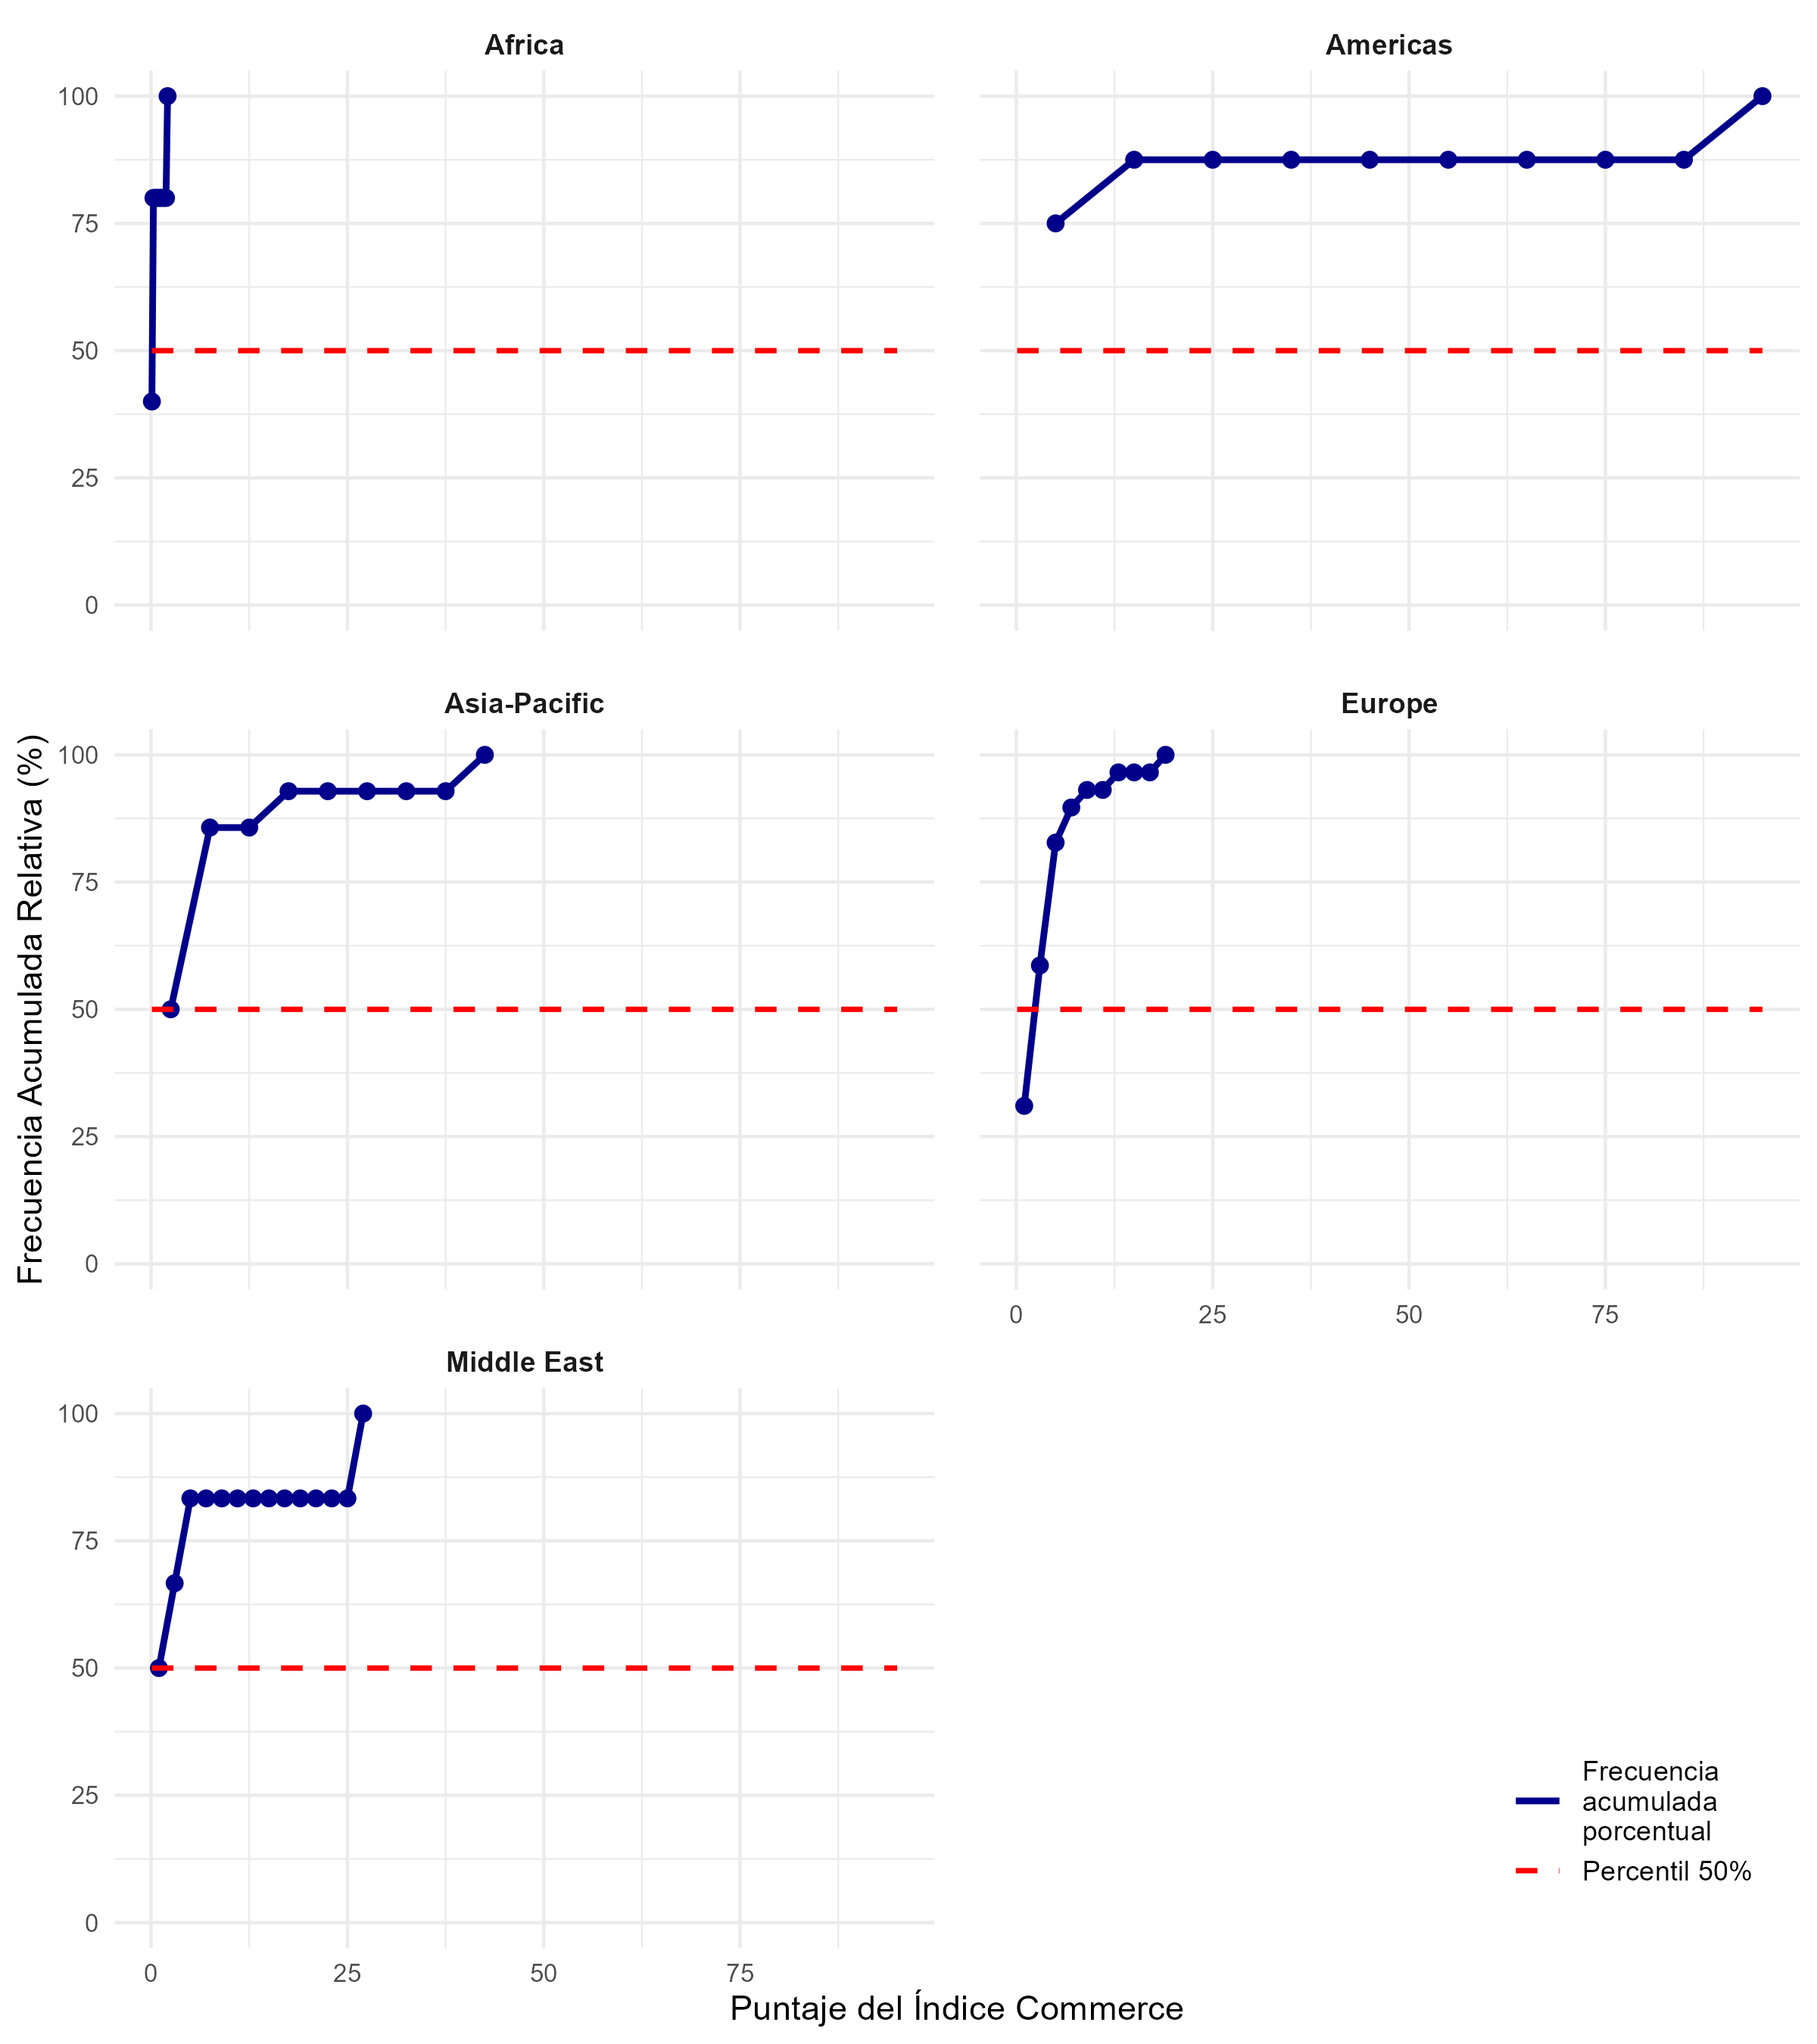
\includegraphics[width=\linewidth]{figura3.png}
\end{center}
Figura 3. Distribución acumulada del Índice Commerce agrupado por Región.


El diagrama de cajas y bigotes presentado en la figura 4



\begin{center}
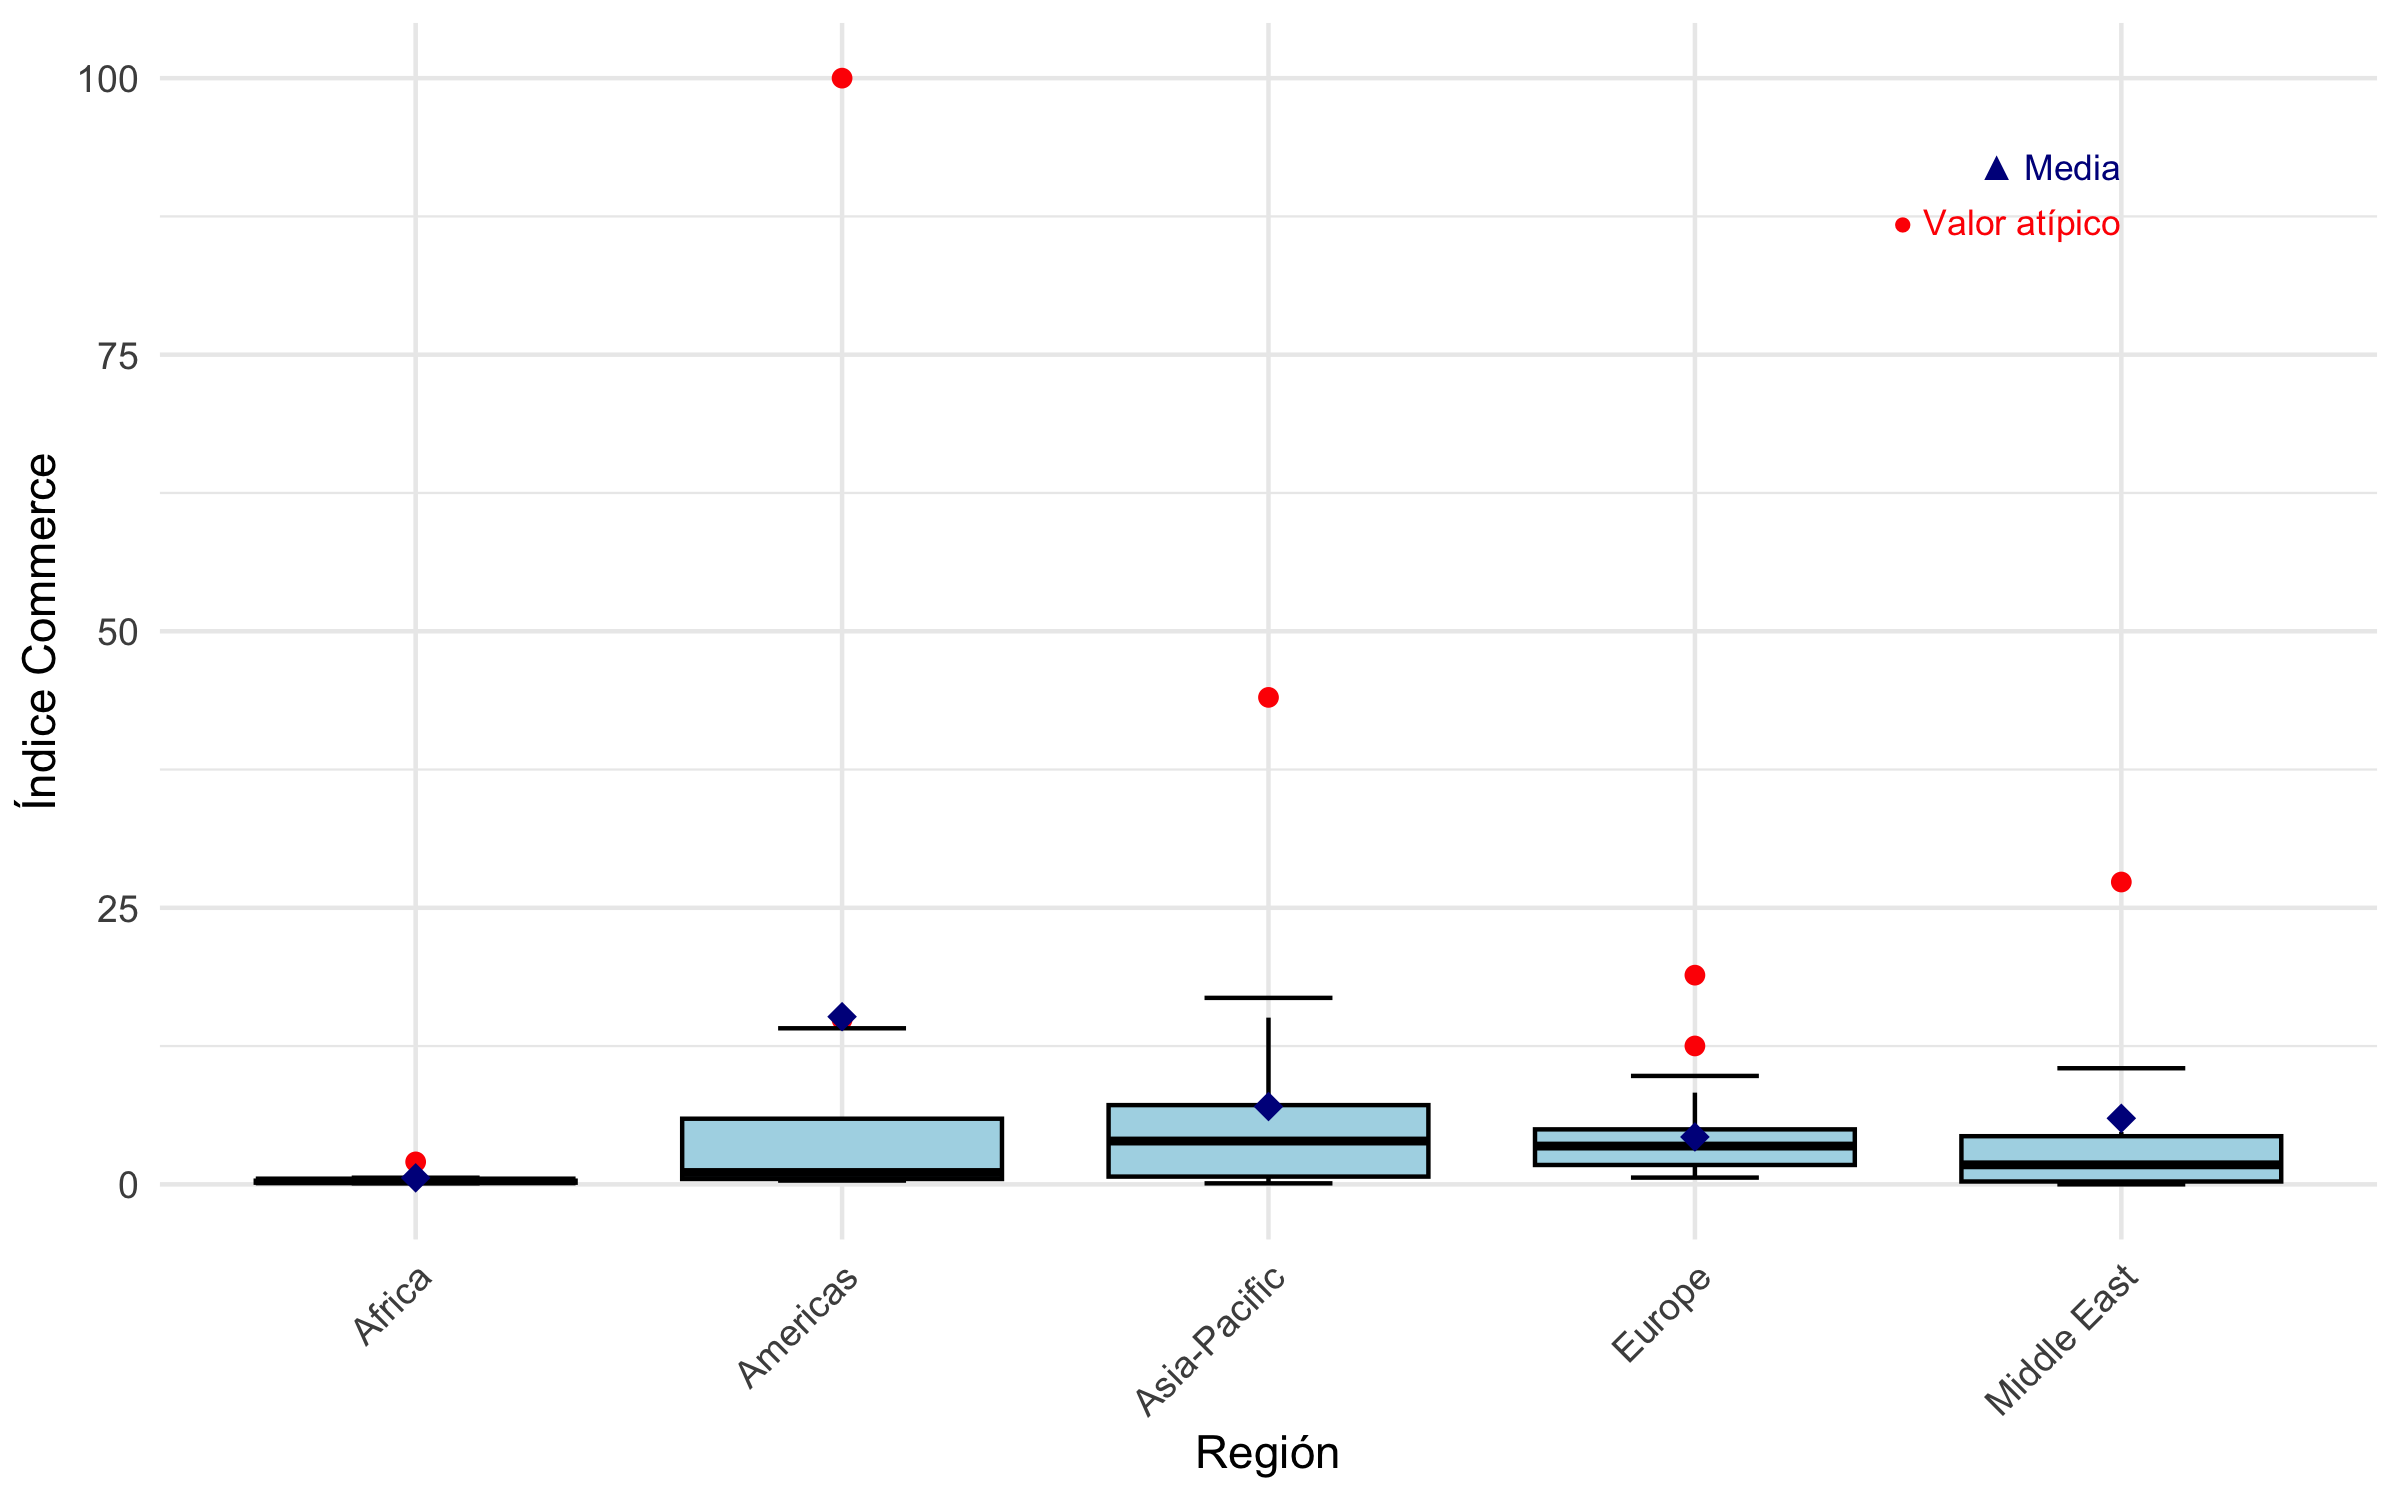
\includegraphics[width=\linewidth]{figura4.png}
\end{center}
Figura 4. Distribución de las medidas de posición del Índice Commerce agrupado por Región.


\subsection{Índice Research}
tabla de frecuencia bivariada (indice vs total socore)
histograma x region
ojiva x region
diagrama de cajas y bigotes x region


\subsection{Índice Talent}
tabla de frecuencia bivariada (indice vs total socore)
histograma x region
ojiva x region
diagrama de cajas y bigotes x region

\subsection{Región}
tabla de frecuencia univariada de los índices discriminados por región
tabla de frecuencia bivariada (region y total score)
diagrama de barras
diagrama de torta

\section{Análisis de resultados}

\section{Conclusiones}

\section{Referencias}
[1]   “AI Global Index,” Kaggle, Apr. 26, 2023.         https://www.kaggle.com/datasets/katerynameleshenko/ai-index

[2]   W. Navidi, Statistics for Engineers and Scientists w/ CD-ROM. McGraw-Hill Sci./Eng./Math, 2004.

\end{multicols}

\end{document}
